\NextFile{ui.html}

\chapter{Front Panel Operation}\label{chap:whatever}

Since 2012, MakerBot printers and their clones have included a built in user
interface comprised of a \gls{LCD} screen and a five-button keypad.  With this
user interface, the printer can be operated without the use of a computer.

This chapter describes the operation of Replicator-style printers through this
built-in interface.

\ifdefined\luluflag
\else
For users of Thing-o-Matics with ``Gen 4 LCD interfaces'', please refer
to the ``Pages Archive'' of the MakerBot Wiki found at
\myhref{http://www.makerbot.com/support/archive/}{http://www.makerbot.com/support/archive/}.  There, documentation for the Thing-o-Matic
LCD interface may be found as part of the ``\gls{Jetty Firmware}''
documentation.
\fi

\NextFile{ui-splash.html}

\section{Splash Screen}\label{sec:Splash}
\index{Screens!Splash}

Every time you power on your printer, the \gls{LCD} screen should be similar to the one pictured in Figure~\ref{fig:splash}.  This splash screen only lasts for a few seconds, so you may miss seeing it.

\begin{figure}[!htbp]
  \centering
    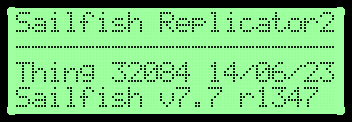
\includegraphics[]{splash-01}
    \caption{Splash Screen}
  \label{fig:splash}
\end{figure}

If, however, you should instead see a screen with two horizontal black bars (as pictured in Figure~\ref{fig:error}), then your printer either does not have \gls{firmware} loaded or has an electrical problem.\index{LCD!Solid bars}

\begin{figure}[!htbp]
  \centering
    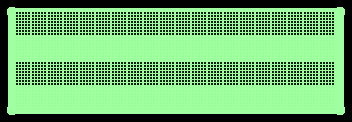
\includegraphics[]{splash-02}
    \caption{Bad News}
  \label{fig:error}
\end{figure}

The splash screen contains the following information:

\begin{enumerate}
\item The \myhref{http://www.thingiverse.com/thing:32084}{Thingiverse ``Thing'' number 32084}.
\item The type of microprocessor in your printer: an ATmega~1280 or 2560.
\item The date the firmware was built in year/month/day format.
\item The version and revision numbers.
\end{enumerate}

If you miss seeing the splash screen, much of this information may also be found in the ``Version Information'' item under the ``Utilities'' menu, Section~\ref{sec:versinf}.

After a few seconds, the splash screen is dismissed and replaced by the main
\ifpdf
menu.
\else
menu, Section~\ref{sec:Main}.
\fi

\NextFile{ui-main-menu.html}

\section{Main Menu}\label{sec:Main}
\index{Menus!Main}

The main menu (Figure~\ref{fig:main}) is your base of operations.  When it appears, the screen should have a title line displaying the name of the printer; you may change this name with either ReplicatorG or MakerWare.  The next three lines allow you to print from a memory card (i.e., an \gls{SD card}), preheat your printer, and access the printer's utilities.  

\begin{figure}[!htbp]
  \centering
    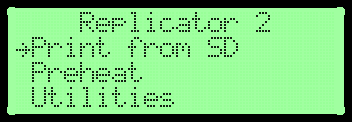
\includegraphics[]{main-01}
    \caption{Main Menu}
  \label{fig:main}
\end{figure}

You navigate the menus by using the keypad (Figure~\ref{fig:keypad})  on the front of the printer, which is generally located near the LCD screen:\index{Keys!Keypad}\index{Buttons|see {Keys}}\index{Menus!Navigating}

\begin{figure}[!htbp]
  \centering
\ifpdf
    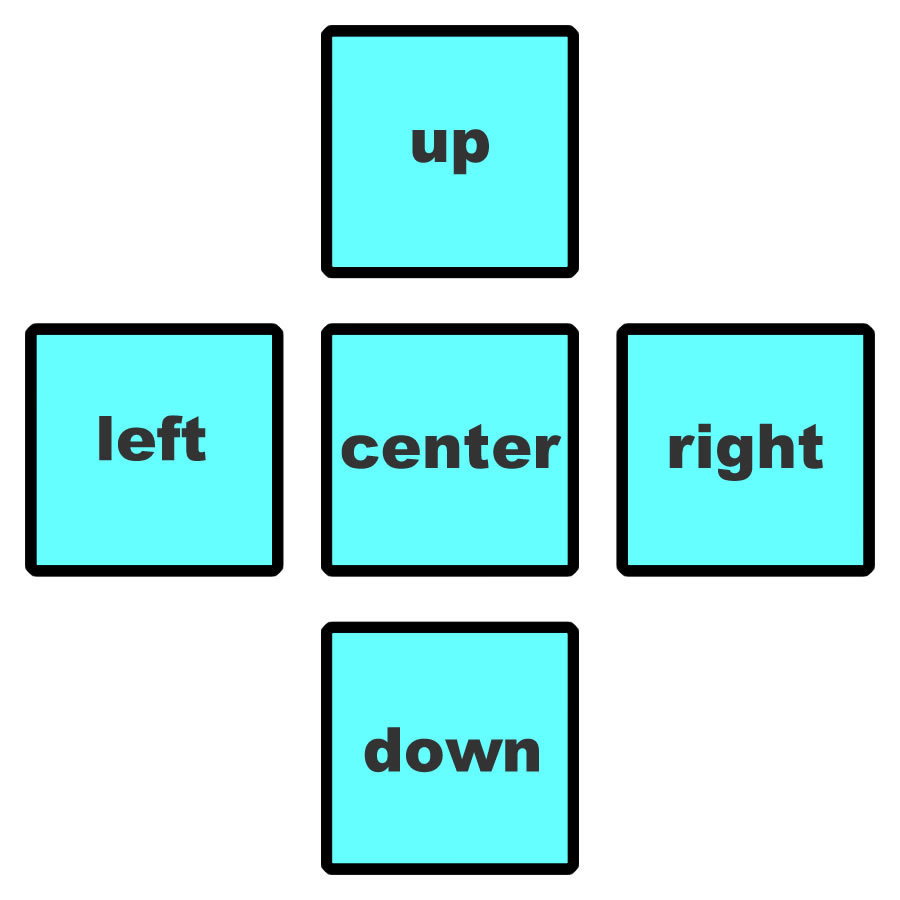
\includegraphics[]{keypad}
\else
    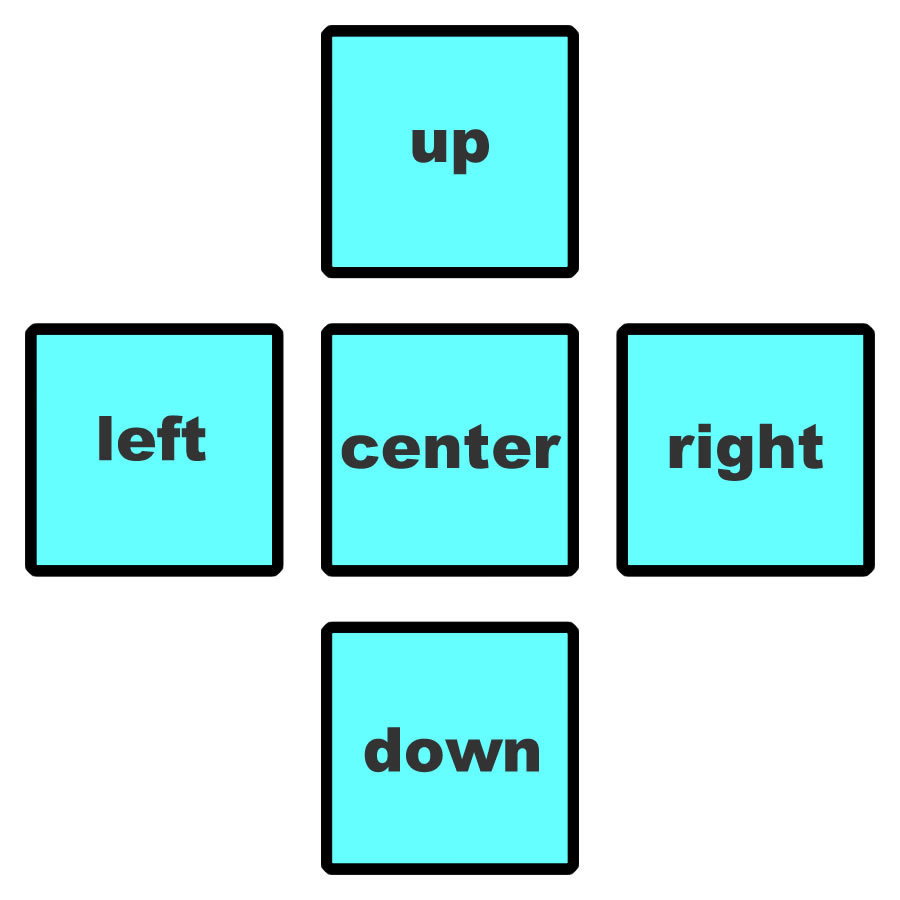
\includegraphics[width=3in]{keypad}
\fi
    \caption{Keypad}
  \label{fig:keypad}
\end{figure}

\begin{enumerate}
\item The up and down keys allow you to scroll through the list, which wraps around (so, if you scroll down from the bottom of the list you will return to the top of the list).\index{Keys!Up}\index{Keys!Down}
\item The center key (which, on some printers, has an ``M'' printed on it) allows you to select the item that has an arrow pointing to it.  In Figure~\ref{fig:main} this is the ``Print from SD'' item.  You can also dismiss any error message by pressing this key, which will then return you to the main menu.\index{Keys!Center}
\item The left key allows you to exit a menu and return to the previous menu.  Note that many menus have an ``Exit Menu'' option that will also return you to the previous menu.\index{Keys!Left}
\item Within the Jog Mode (Section~\ref{sec:jog}), Profiles: Change Name (Section~\ref{sec:profiles}), and Pause at ZPos (Section~\ref{sec:zpos}) menus where the right key is used, its function is described.  Otherwise, pressing the right key will reinitialize and repaint the LCD screen.\index{Keys!Right}
\end{enumerate}

\ifpdf
Table~\ref{tab:menu-tree} outlines the hierarchy of menus accessible through the front panel.
\fi

\ifpdf
\ifdefined\htmlflag
\else
\noindent
{\relsize{-1}
\begin{table}[!hb]
\begin{tabular}{lllll}
\hhline{~~|-|~~}
&& \cellcolor{LightBlue} \hyperref[sec:printmon]{Return to Monitor} \\
\hhline{~~|-|~~}
&& \cellcolor{LightBlue!50} \hyperref[sec:cancel]{Cancel Print} \\
\hhline{~~|-|~~}
&& \cellcolor{LightBlue} \hyperref[sec:pause]{Pause} \\
\hhline{~~|-|~~}
&& \cellcolor{LightBlue!50} \hyperref[sec:zpos]{Pause at ZPos} \\
\hhline{~~|-|~~}
&& \cellcolor{LightBlue} \hyperref[sec:speed]{Change Speed} \\
\hhline{~~|-|~~}
&& \cellcolor{LightBlue!50} \hyperref[sec:temp]{Change Temperature} \\
\hhline{~~|-|~|-|}
&& \cellcolor{LightBlue} \hyperref[sec:cooling]{Set Cooling Fan} && \cellcolor{LightCyan} \hyperref[sec:ditto]{Ditto Printing} \\
\hhline{~~|-|~|-|}
&& \cellcolor{LightBlue!50} \hyperref[sec:printstat]{Print Statistics} && \cellcolor{LightCyan} \hyperref[sec:override]{Override GcTemp} \\
\hhline{|-|-|-|~|-|}
\multicolumn{2}{l}{\cellcolor{LightBlue} \hyperref[sec:sdmenu]{Print from {\relsize{-0.5}SD}} \hfil $\Longrightarrow$ \hfil} & \cellcolor{LightBlue} \hyperref[sec:cold]{Cold Pause} && \cellcolor{LightCyan} \hyperref[sec:pauseheat]{Pause with Heat} \\
\hhline{|-|-|-|~|-|}
\cellcolor{LightCyan} \hyperref[sec:preheat]{Preheat} \phantom{om SD} &&&& \cellcolor{LightCyan} \hyperref[sec:sound]{Sound}  \\
\hhline{|-|-|-|~|-|}
\multicolumn{2}{l}{\cellcolor{LightBlue} \hyperref[sec:utilities]{Utilities} \hfil\phantom{mmm}\hfil $\Longrightarrow$} & \cellcolor{LightBlue} \hyperref[sec:monmode]{Monitor Mode} && \cellcolor{LightCyan} \hyperref[sec:acceleration-enable]{Acceleration} \\
\hhline{|-|-|-|~|-|}
&& \cellcolor{LightCyan} \hyperref[sec:filload]{Filament Loading} && \cellcolor{LightCyan} \hyperref[sec:extruder-count]{Extruder Count} \\
\hhline{~~|-|~|-|}
&& \cellcolor{LightBlue} \hyperref[sec:preheatset]{Preheat Settings} && \cellcolor{LightCyan} \hyperref[sec:extruder-hold]{Extruder Hold} \\
\hhline{~~|-|-|-|}
&& \multicolumn{2}{l}{\cellcolor{LightCyan} \hyperref[sec:general]{General Settings} \hfil\phantom{mmm} \hfil $\Longrightarrow$} & \cellcolor{LightCyan} \hyperref[sec:hbp-present]{HBP Installed} \\
\hhline{~~|-|-|-|}
&& \cellcolor{LightBlue} \hyperref[sec:levelbp]{Level Build Plate} && \cellcolor{LightCyan} \hyperref[sec:sd-crc]{Check SD Reads} \\
\hhline{~~|-|~|-|}
&& \cellcolor{LightCyan} \hyperref[sec:home-axes]{Home Axes} && \cellcolor{LightCyan} \hyperref[sec:pstop-enable]{P-Stop Control} \\
\hhline{~~|-|~~}
&& \cellcolor{LightBlue} \hyperref[sec:bot-stats]{Bot Statistics} \\
\hhline{~~|-|~~}
&& \cellcolor{LightCyan} \hyperref[sec:filodo]{Filament Odometer} \\
\hhline{~~|-|-|-|}
&& \multicolumn{2}{l}{\cellcolor{LightBlue} \hyperref[sec:profiles]{Profiles} \hfil\phantom{nmmmmmmm} \hfil $\Longrightarrow$} & \cellcolor{LightBlue} \hyperref[sec:profiles-r]{Restore} \\
\hhline{~~|-|-|-|}
&& \cellcolor{LightCyan} \hyperref[sec:homeoff]{Home Offsets} && \cellcolor{LightBlue} \hyperref[sec:profiles-dc]{Display Config} \\
\hhline{~~|-|~|-|}
&& \cellcolor{LightBlue} \hyperref[sec:tooloff]{Toolhed Offsets} && \cellcolor{LightBlue} \hyperref[sec:profiles-cn]{Change Name} \\
\hhline{~~|-|~|-|}
&& \cellcolor{LightCyan} \hyperref[sec:jog]{Jog Mode} && \cellcolor{LightBlue} \hyperref[sec:profiles-sp]{Save to Profile} \\
\hhline{~~|-|~|-|}
&& \cellcolor{LightBlue} \hyperref[sec:steppers-enable]{Enable/Disable Steppers} \\
\hhline{~~|-|~~}
&& \cellcolor{LightCyan} \hyperref[sec:alevel-variance]{Auto-level Variance} \\
\hhline{~~|-|~~}
&& \cellcolor{LightBlue} \hyperref[sec:alevel-maxhits]{Max Z Probe Hits} \\
\hhline{~~|-|~~}
&& \cellcolor{LightCyan} \hyperref[sec:calibnozz]{Calibrate Nozzles} \\
\hhline{~~|-|~~}
&& \cellcolor{LightBlue} \hyperref[sec:restore-settings]{Restore Settings} \\
\hhline{~~|-|~|-|}
&&  \multicolumn{2}{l}{\cellcolor{LightCyan} \hyperref[sec:eeprom]{EEPROM} \hfil\phantom{nmmmmmm} \hfil $\Longrightarrow$} & \cellcolor{LightCyan} \hyperref[sec:eeprom]{Eeprom -\textgreater\ SD} \\
\hhline{~~|-|~|-|}
&& \cellcolor{LightBlue} \hyperref[sec:versinf]{Version Information} && \cellcolor{LightCyan} \hyperref[sec:eeprom]{SD -\textgreater\ Eeprom} \\
\hhline{~~~~|-|}
&&&& \cellcolor{LightCyan} \hyperref[sec:eeprom]{Erase Eeprom} \\
\hhline{~~~~|-|}
\end{tabular}
\caption[Front panel menu hierarchy]{Front panel menu hierarchy}
\label{tab:menu-tree}
\end{table}
}
\fi
\fi


\NextFile{ui-print-from-sd-menu.html}

\section{Print from SD Menu}\label{sec:sdmenu}
\index{Menus!Print from SD}
\index{SD card}
\index{Flashcard|see {SD card}}
\index{Printing!Starting a print}

This menu allows you to print items you have already saved on an \gls{SD card} (also called a flashcard), which provides you the ability to print without connecting your printer to a computer.  When you open this menu, you should see a list of the items saved on your SD card.  An example menu is shown in Figure~\ref{fig:sdmenu}.  The last item on the menu is an ``Exit Menu'' shortcut that will return you to the main menu.

\begin{figure}[!htbp]
  \centering
    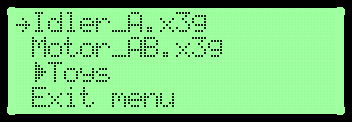
\includegraphics[]{printsd-01}
    \caption{SD Menu}
  \label{fig:sdmenu}
\end{figure}

\ifpdf
\ifdefined\luluflag
\else
\pagebreak[4]
\fi
\fi

If instead, you see the error message ``SD card not present'' then you need to insert an SD card into your printer.\index{Errors!SD card not present}

If the error message ``Unable to read this SD card format.  Reformat as FAT-16 or FAT-32'' is displayed, then you need to remove your SD card and reformat it.\index{Errors!Unable to read this SD card format...}  The SD card \emph{must} be formatted as \gls{FAT-16}.\index{SD card!Format}  Unlike standard MakerBot firmware (which only supports FAT-16 on SDSC cards of 2 GB or less), any capacity of SD card may be used, including SDSC (standard capacity), SDHC (high capacity), and SDXC (extended capacity) cards.  Note that many new SD cards now come formatted using the proprietary, licensed ``eFAT'' format.  Sailfish does not support this format as implementation requires licensing from Microsoft.  If you have difficulty with a new SD card, you may wish to check its format on your computer, reformatting it as ``FAT'' if necessary.

To print an item, scroll to it and then press the center key; this will start the printing of the model, displaying the print monitor screen. %name  
\index{SD card!Files not appearing|(}If you are unable to see or print an item saved on your card, you should reformat the files on the SD card.  Items should be saved as \glspl{X3G} or \glspl{S3G} files (not case sensitive) with filenames 31 or fewer characters including extension. It is best to use simple filenames that do not include spaces, accents, or other special characters.\index{SD card!File names}\footnote{Note that \texttt{.s3g} is an older type of file, so you may wish to consider regenerating any \texttt{.s3g} files on your computer as \texttt{.x3g} files.}

If you are still unable to find an item, it may be in a folder.  In Figure~\ref{fig:sdmenu} the item ``Toys'' is a folder, as indicated by the solid triangle.\index{SD card!Folders}
Folders can be opened by pressing the center key, which will take you to a submenu (See Figure~\ref{fig:submenu}).  For this reason, folders are useful organizational tools if you have many items on your SD card.\index{SD card!Files not appearing|)}

\begin{figure}[!htbp]
  \centering
    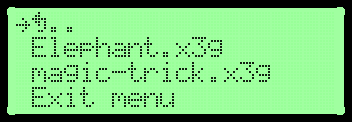
\includegraphics[]{printsd-02}
    \caption{SD ``Toys'' Submenu}
  \label{fig:submenu}
\end{figure}

Note that if you either press the left key or select the return symbol from within a folder, you return to the previous folder or screen, while the ``Exit Menu'' shortcut returns you to the main menu.  For your convenience, if you have returned to the main menu from the ``Exit Menu'' shortcut, when you return to the ``Print from SD'' menu, you return to whichever folder you had been in.  Note that if you remove the SD card and reinsert it this folder state is lost.  Likewise, the folder state is lost when you power off your printer.

\NextFile{ui-print-monitor-menu.html}

\section{Starting a Print: the Print Monitor \& Menu}\label{sec:printmon}
\index{Printing!Starting a print}
\index{Printing!Monitor screen}
\index{Screens!Print monitor}

Once you start a print from the ``Print from SD'' menu (Section~\ref{sec:sdmenu}), the LCD screen should display the print monitor.  By pressing the center key you can exit the print monitor to access the print menu.

If you have not preheated your printer, the screen will display a heating progress bar on the first line, as seen in Figure~\ref{fig:printpreheat}.

\begin{figure}[!htbp]
  \centering
    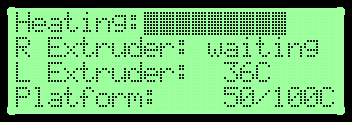
\includegraphics[]{printing-02}
    \caption{Print Monitor --- Preheating}
  \label{fig:printpreheat}
\end{figure}
  
The screen should also display the current temperatures and target temperatures (in Celsius) of all your heating elements in the form current temperature/target temperature --- if, however, the element is not going to be heated, then it will only display its current temperature.  Note that for some printers the extruders do not start heating until the platform has heated (such as genuine MakerBots with smaller power supplies).  In this case the screen will display ``waiting'' rather than the temperatures.\index{Waiting temperature}  In addition, the number of heating elements displayed will depend on the number your printer has.  Figure~\ref{fig:printpreheat} shows a dual extruder set-up.

Once your printer has finished heating, it will play a short tune to inform you and the heating progress bar will be replaced by a line displaying the name of the print (which will be the name on the SD card unless print commands in the file change the displayed name) and the percentage completed of the print (Figure~\ref{fig:print}).  Since the percentage is generated by the \gls{slicer}, it will remain displayed as 0\% if the file does not contain print commands to update it.  If a future Pause at Z-Position is scheduled (Section \ref{sec:zpos}), then an asterisk will appear before the percentage.\index{Percentages, build}

\begin{figure}[!htbp]
  \centering
    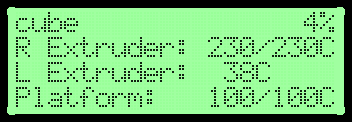
\includegraphics[]{printing-03}
    \caption{Print Monitor --- Printing}
  \label{fig:print}
\end{figure}

On \emph{some} printers with only two heating elements the firmware uses the extra available line to display a running ticker of statistics:\index{Printing!Ticker display}
\begin{enumerate}
\item The elapsed build time.\index{Printing!Elapsed time}
\item The estimated build time remaining.  This will only be generated if the print commands include the percentage complete updates and is, therefore, only as accurate as the percentage markers.\index{Printing!Estimated time left}
\item The current filament usage.\index{Printing!Filament usage}\index{Filament!Usage}
\item The current Z position.\index{Printing!Current build height}
\end{enumerate}
If this ticker is not displayed, the information can be accessed in the ``Print Statistics'' item under the print menu, Section~\ref{sec:printstat}.

By pressing the center key to dismiss the print monitor, you can access the print menu, seen in Figure \ref{fig:printeth-menueth}.

\begin{figure}[!htbp]
  \centering
    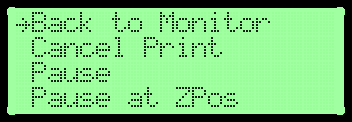
\includegraphics[]{printing-04}
    \caption{The first screen of the print menu}
  \label{fig:printeth-menueth}
\end{figure}

The print menu allows you to control aspects of the printing process as well as monitor the printing progress:\index{Menus!Print menu}
\begin{enumerate}
\item Back to Monitor: returns you to the print monitor.
\item Cancel Print: as the name suggests, this allows the termination of the print.  A confirmation screen will be generated to prevent accidental termination.
\item Pause: by allowing you to suspend a print and generating the pause menu, the pause option lets you change aspects of the print.  If the printer is left paused for over 30 minutes the heaters will turn off even if ``Pause with Heat'' is enabled (Section~\ref{sec:pauseheat}).
\item Pause at ZPos: lets you program the print to stop at a certain height.  Once the printer pauses, the pause menu will be generated.  Again, if the printer is left paused for over 30 minutes the heaters will turn off even if ``Pause with Heat'' is enabled.\footnote{Commands to pause at specified heights may be placed directly in a print file; see Section~\ref{sec:special-gcode}.}
\item Change Speed.
\item Change Temperature.
\item Change HBP Temp: this item only appears if your printer is equipped with a heated build plate. 
\item Set Cooling Fan ON/OFF.
\item Set Lights OFF/ON.
\item Print Statistics: displays the elapsed build time, the estimated build time remaining for prints with percentage complete updates, the current filament usage, and the current Z position. 
\item Cold Pause: pauses, cools off all heating elements, turns off LED lighting, and generates the pause menu.
\end{enumerate}

\NextFile{ui-print-monitor-menu-cancel-print.html}

\subsection{Cancel Print}\label{sec:cancel}
\index{Printing!Canceling}

To cancel a print while printing, choose the ``Cancel Print'' item under the print menu.  Do not just turn off the printer, as that can damage the printer.  Choosing this item will generate the confirmation screen pictured below in Figure~\ref{fig:cancel}.

\begin{figure}[!htbp]
  \centering
    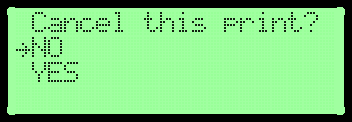
\includegraphics[]{printing-05}
    \caption{Cancel Print Confirmation}
  \label{fig:cancel}
\end{figure}

Once you have canceled the print, the printer will cease printing and move your print away from the extruders by lowering the build platform.  All the heaters will be switched off.

\NextFile{ui-print-monitor-menu-pause.html}

\subsection{Pause}\label{sec:pause}
\index{Printing!Pausing}
\index{Pausing}

Pausing your printer generates the pause menu, which allows you to change aspects of the print that cannot otherwise be changed in the middle of printing.  The pause is not immediate, as the printer will continue printing until it clears out its buffer of queued work.  The LCD screen will acknowledge this and generate the screen as seen in Figure~\ref{fig:clear}.  Note that, once paused, the build platform will automatically lower by 5 mm.

\begin{figure}[!htbp]
  \centering
    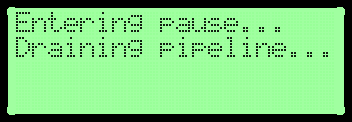
\includegraphics[]{pause-drain}
    \caption{Clearing Queue}
  \label{fig:clear}
\end{figure}

When your printer starts to pause, you should see the screen shown in Figure~\ref{fig:startpause}.

\begin{figure}[!htbp]
  \centering
    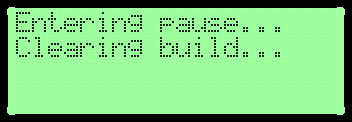
\includegraphics[]{pause-clear}
    \caption{Pause}
  \label{fig:startpause}
\end{figure}

Once your printer is paused, the pause menu appears:\index{Menus!Pause}

\begin{enumerate}
\item Jog Mode: shift the platform or extruder along the X, Y, and Z axes.  Be careful not to hit the endstops, as that will cause a loss of registration and the print will not resume in the proper place.  The jog mode is identical to ``Jog Mode'' in the ``Utilities'' menu; for operation details see Section~\ref{sec:jog}.
\item Filament Loading: allows you to load and unload filament.  As this is identical to ``Filament Loading'' in the ``Utilities'' menu, see Section~\ref{sec:filload}.
\item Heaters Off: turns off all heaters.  Again, note that if the printer is paused for over 30 minutes the heating units should turn off automatically even if ``Pause with Heat'' is enabled, Section~\ref{sec:pauseheat}.
\end{enumerate}

To resume printing select the ``Unpause'' item on the pause menu.  You should see the screen pictured in Figure~\ref{fig:endpause}.\index{Printing!Resuming}  Note that if the print has been paused for an extended period, it is best to run the filament load for 10--30 seconds to purge the extruder of cooked plastic.  If the extruder is sitting over your print, use the jog controls to move it over a clear spot.  

\begin{figure}[!htbp]
  \centering
    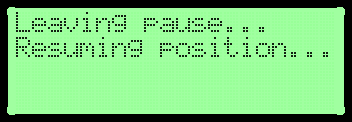
\includegraphics[]{unpause-resume}
    \caption{Unpause}
  \label{fig:endpause}
\end{figure}

\NextFile{ui-print-monitor-menu-pause-at-zpos.html}

\subsection{Pause at ZPos}\label{sec:zpos}
\index{Pause at ZPos}
\index{Printing!Pausing at a set height}
\index{Printing!Pause @ ZPos}
\index{Pausing!Specified build height}

This programs the printer to pause when it first attains or exceeds a specified height.  Choosing this item will generate the screen depicted in Figure~\ref{fig:Zpause}.

\begin{figure}[!htbp]
  \centering
    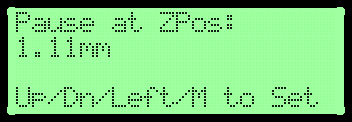
\includegraphics[]{printing-10}
    \caption{Pause at ZPos}
  \label{fig:Zpause}
\end{figure}

To change the Z position use the up and down keys, and to set the Z position press the center key.  Pressing the right key once changes the Z position in larger increments, a second causes larger increment still, but a third time will set the value by which it increments back to the original; it is actually doing this in units of steps, but still displays units of millimeters.  Pressing the left key cancels any changes to the Pause at Z-Position value.

Note that the printer continues printing while you set the Z position.

Since you can include multiple pauses at specified Z positions within the printing file, the printer honors the last pause it has received.  Therefore, if it encounters a pause within the printing file after you manually set one, it will replace the Pause at Z-Position that you have set with the one in the print file.  Likewise, if you have included pauses within the print file, they will be replaced by any subsequent pauses you enter manually.

If you set a Pause at Z-Position and later wish to cancel any such pause you can either allow it to pause and then manually resume right after, or set the Z position for the pause to a value not attained by the print.  Note that each print starts without a Pause at Z-Position set --- the changes are not retained between prints.

When using Pause at ZPos it is important to note that the \gls{slicer} probably started your model a few hundredths of a millimeter above zero so you need to account for this difference when setting a pause height.

Once the print has attained the specified height, the pause menu (Section~\ref{sec:pause}) will be generated and the build platform will be lowered by 5 mm.

\NextFile{ui-print-monitor-menu-change-speed.html}

\subsection{Change Speed}\label{sec:speed}
\index{Printing!Changing speed}

This item allows you to change the printing speed by a multiplicative factor (see Figure~\ref{fig:speed}).  \emph{As you enter the speed}, it starts percolating through the queue of already buffered work.

\begin{figure}[!htbp]
  \centering
    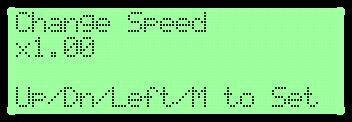
\includegraphics[]{printing-12}
    \caption{Change Speed}
  \label{fig:speed}
\end{figure}

To increase the speed use the up key, and to decrease it use the down key.  The center key will set the speed and return you to the print menu while the left key will cancel any changes and return you to the print menu.  Note that pressing the left key will \emph{not} necessarily return the speed to 1.00, rather, it reinstates the scaling factor which was in effect when the screen was entered.

\NextFile{ui-print-monitor-menu-change-temperature.html}

\subsection{Change Temperature}\label{sec:temp}
\index{Printing!Changing temperature}

This allows you to change the temperature of the currently active extruder while printing.  You cannot use this menu (see Figure~\ref{fig:printtemp}) to change the heated platform's temperature or the temperature of an inactive extruder.

\begin{figure}[!htbp]
  \centering
    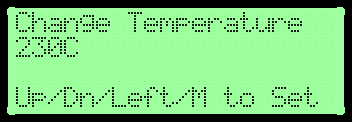
\includegraphics[]{printing-13}
    \caption{Change Temperature}
  \label{fig:printtemp}
\end{figure}

To increase the temperature use the up key; to decrease it use the down key.  You cannot set the temperature above 280\textdegree\,C and, naturally, you also do not wish to set it too low or else the filament will not melt.

Unlike the change speed item, the temperature changes do not take effect until the center key is pressed.  Pressing this key sets the temperature and returns you to the print menu.  Note that if you change the temperature by more than 10\textdegree\,C at a time the algorithm used by the temperature control will reset, which can cause temperature instability for upwards of a minute.  Pressing the left key cancels any change in temperature, resetting the temperature to what it had been, and returns you to the print menu.

\NextFile{ui-print-monitor-menu-change-hbp-temp.html}

\subsection{Change HBP Temp}\label{sec:hbp-temp}
\index{Printing!Changing the temperature for the heated build platform}

If you have a heated build platform installed, this menu (see Figure~\ref{fig:printhbptemp})  will appear to allow you to change the temperature of the platform while printing. You cannot use this menu to change the temperature of any of the extruders.

\begin{figure}[!htbp]
  \centering
    \includegraphics[]{printing-09}
    \caption{Change HBP Temperature}
  \label{fig:printhbptemp}
\end{figure}

To increase the temperature use the up key; to decrease it use the down key.  Note that you cannot set the temperature above 130\textdegree\,C.

Similar to the change temperature item, the temperature changes for the heated platform do not take effect until the center key is pressed, which will then set the temperature and return you to the print menu.  Again, note that if you change the temperature by more than 10\textdegree\,C at a time the PID state is reset, which can cause a wide temperature swing.  While increments of about 5\textdegree\,C work best, any value of 10\textdegree\,C or less will work. Pressing the left key cancels any change in temperature, resetting the temperature to what it had been, and returns you to the print menu.

If you do not see this menu option despite having a heated build platform installed, you will need to navigate to the ``HBP Installed'' option under the ``General Settings'' menu of the ``Utilities'' menu when you are done printing, which is discussed in Section~\ref{sec:hbp-present}.

\NextFile{ui-print-monitor-menu-set-cooling-fan.html}

\subsection{Set Cooling Fan}\label{sec:cooling}
\index{Cooling fan}
\index{Printing!Cooling fan}

This allows you to change the state of the \gls{print cooling fan} on printers that have such a fan.  Note that this has nothing to do with the \glspl{heatsink cooling fan}.  If the cooling fan is currently off, then the option will read ``Set Cooling Fan ON'' as depicted in Figure~\ref{fig:coolingfan} below.  Likewise, if the cooling fan is on, then the option will read ``Set Cooling Fan OFF''.

\begin{figure}[!htbp]
  \centering
    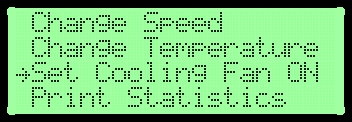
\includegraphics[]{printing-15}
    \caption{Set Cooling Fan}
  \label{fig:coolingfan}
\end{figure}

Note that some \glspl{slicer} generate many commands to turn the fan on and off throughout the course of the print.  When you turn the fan on or off with this item, any subsequent print commands to change the fan's state \emph{will} be honored --- this option does not override all further print commands regarding the fan.

\NextFile{ui-print-monitor-menu-set-lights.html}

\subsection{Set Lights}\label{sec:printsetlights}
\index{Printing!Lights}

This option allows you to change the state of the printer's LED lights mid-print if necessary. If the lights are currently on, then the option will read ``Set Lights OFF''. Similarly, if the lights are off, then the option will read ``Set Lights ON''. You can change this state by scrolling to the option and pressing the center key.

\NextFile{ui-print-monitor-menu-print-statistics.html}

\subsection{Print Statistics}\label{sec:printstat}
\index{Printing!Statistics}

This item (Figure~\ref{fig:printstatistics}) allows you to see the progress of the print as reflected in four items:
\begin{enumerate}
\item Print Time: the elapsed build time.\index{Printing!Elapsed time}
\item Time Left: the estimated build time remaining.  This will only be generated if the print commands include percentage complete updates and is, therefore, only as accurate as the percentage markers.\index{Printing!Estimated time left}
\item Filament: the length of filament used so far in meters.\index{Printing!Filament usage}\index{Filament!Usage}
\item ZPosition: the current Z position in mm.\index{Printing!Current build height}
\end{enumerate}

\begin{figure}[!htbp]
  \centering
    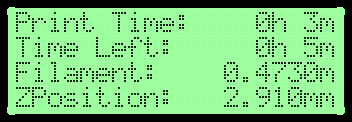
\includegraphics[]{printing-14}
    \caption{Print Statistics}
  \label{fig:printstatistics}
\end{figure}

If your firmware has auto-leveling, then the last line will alternate between auto-leveling status and Z position, displaying one for a few seconds and then the other.

\NextFile{ui-print-monitor-menu-cold-pause.html}

\subsection{Cold Pause}\label{sec:cold}
\index{Printing!Cold pause}
\index{Pausing!Cold}

This option allows you to pause the print and automatically turn off the heaters and LEDs.  This will also generate the pause menu, Section~\ref{sec:pause}, and lower the build platform by 5 mm.

\NextFile{ui-completing-a-print.html}

\section{Completing a Print} \label{sec:print-done}

Once the print is completed, the LCD generates a screen similar to the one shown in Figure~\ref{fig:printcomplete}.

\begin{figure}[!htbp]
  \centering
    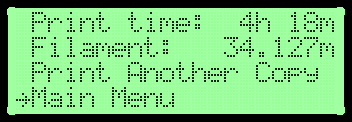
\includegraphics[]{finish-01}
    \caption{Print From SD Card Complete}
  \label{fig:printcomplete}
\end{figure}

This screen shows how long the print took (in hours and minutes) and how much filament was used (in meters).  You are also given the options of either reprinting the item or returning to the main menu.  If you choose to print another copy, you \emph{must} first clear the build plate before selecting ``Print Another Copy'', as the reprint will then begin \emph{immediately}.  Note that pressing the left key will also return you to the main menu.

If you instead printed over USB, you should see a screen similar to the one in Figure~\ref{fig:usbprint} below.  The only difference is that the option of printing another copy is not available.

\begin{figure}[!htbp]
  \centering
    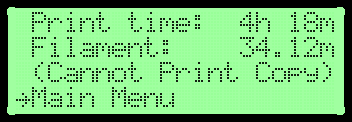
\includegraphics[]{finish-02}
    \caption{Print From USB Complete}
  \label{fig:usbprint}
\end{figure}

\NextFile{ui-preheat-menu.html}

\section{Preheat Menu}\label{sec:preheat}
\index{Menus!Preheat}
\index{Preheat}
\index{Printing!Preheat}

This menu can be used to begin heating your printer without starting printing.  Doing this directly before starting a print will reduce the time it takes for the print.  The screen generated varies depending on the number of extruders that your printer has.  A dual extruder set-up should display a screen similar to the one depicted in Figure~\ref{fig:preheat}.  Note that the ``Platform'' line will only appear if your printer is equipped with a heated build platform.\index{Heated build platform!Preheating}

\begin{figure}[!htbp]
  \centering
    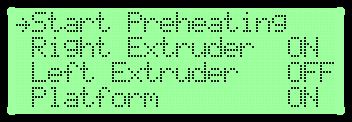
\includegraphics[]{preheat-01}
    \caption{Preheat Menu}
  \label{fig:preheat}
\end{figure}

To turn a heater on or off scroll to its line and then press the center key to toggle it between ``ON'' and ``OFF''.  Then, once you have set which heaters you wish to have on, select the option ``Start Preheating''.\index{Preheat!On}  The enabled heaters will begin heating and the ``Monitor Mode'' screen will be generated.  The ``Monitor Mode'' screen can also be found under the ``Utilities'' menu, and is discussed Section~\ref{sec:monmode}.  This screen should be similar to the one depicted in Figure~\ref{fig:heat}.

\begin{figure}[!htbp]
  \centering
    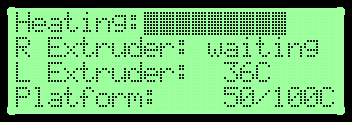
\includegraphics[]{printing-02}
    \caption{Preheating}
  \label{fig:heat}
\end{figure}

The top bar measures the preheating progress.  The current temperatures (in Celsius) of all the heating elements will be displayed next to the target temperatures in the form current temperature/target temperature.  Once the target temperature has been reached, a short tune will be played. The target temperature may be changed in the ``Preheat Settings'' item in the ``Utilities'' menu, Section~\ref{sec:preheatset}.  The screen will display ``waiting'' if an element has not begun heating yet.  Some printers with smaller power supplies, such as genuine MakerBots, do not heat the extruders until the heated build platform has reached temperature.\footnote{Also, MakerWare and Simplify3D will not even send commands to heat the extruders until the heated build platform has finished heating.}

You may dismiss the monitor and return to the main menu by pressing either the center or left key.

If the heaters are already running, then the first line of the Preheat screen will read ``Turn Heaters OFF,'' as shown in Figure~\ref{fig:endheat}.\index{Preheat!Off}

\begin{figure}[!htbp]
  \centering
    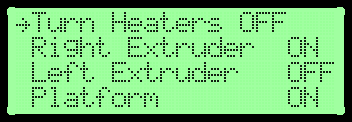
\includegraphics[]{preheat-03}
    \caption{End Preheating}
  \label{fig:endheat}
\end{figure}

By selecting this you turn off \emph{all} the heaters and return to the ``Monitor Mode'' screen, Figure~\ref{fig:heat}.  The first line there will now display the printer's name and the following lines will show only the \emph{current} temperatures.  %image

\NextFile{ui-utilities-menu.html}

\section{Utilities Menu}\label{sec:utilities}
\index{Menus!Utilities}
\index{Utilities}

The utilities menu is accessible from the main menu, Section~\ref{sec:Main}.  Figure \ref{fig:utilitiesfirstscreen} shows the first screen of the utilities menu.

\begin{figure}[!htbp]
  \centering
    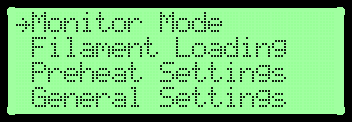
\includegraphics[]{utilities-01}
    \caption{Utilities Menu}
  \label{fig:utilitiesfirstscreen}
\end{figure}

\NextFile{ui-utilities-menu-monitor-mode.html}

\subsection{Monitor Mode} \label{sec:monmode}
\index{Screens!Monitor mode}
\index{Utilities!Monitor mode}

This screen shows you the current temperatures of all your heating elements.  If any of them are enabled, the screen will also show the target temperatures and the heating progress bar as seen in Figure~\ref{fig:heatmonmode}.

\begin{figure}[!htbp]
  \centering
    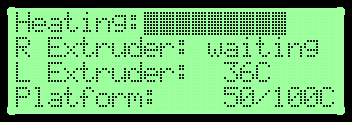
\includegraphics[]{printing-02}
    \caption{Monitor Mode}
  \label{fig:heatmonmode}
\end{figure}

Note that the build platform's current temperature may be as much as 10\textdegree\,C off from that of the extruders when unheated, as the build platform uses a different temperature sensor than the extruders --- one that is more accurate at operating temperatures and less so at room temperature.

\NextFile{ui-utilities-menu-filament-loading.html}

\subsection{Filament Loading} \label{sec:filload}
\index{Utilities!Filament loading}
\index{Filament!Loading}
\index{Filament!Unloading}

This option allows you to load, unload, and change filament in any extruder.  Selecting this option will allow you to choose (if relevant to your printer) which extruder to load or unload.  You will see a screen similar to the one shown in Figure~\ref{fig:filload}, dependent on the number of extruders with which your printer is equipped.

\begin{figure}[!htbp]
  \centering
    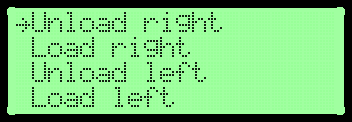
\includegraphics[]{load-01}
    \caption{Filament Loading}
  \label{fig:filload}
\end{figure}

Once you have chosen which extruder for which to change the filament, the printer will begin heating that extruder if necessary, generating a heating progress bar as well as the current and target temperatures, as seen in Figure~\ref{fig:filheat}.  As indicated, press the left key to cancel the operation.  Note that the extruder will be heated up to its preheat temperature, which may be changed in the ``Preheat Settings'' under the ``Utilities'' menu, Section~\ref{sec:preheatset}.

\begin{figure}[!htbp]
  \centering
    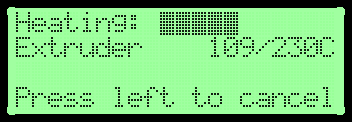
\includegraphics[]{load-03}
    \caption{Extruder Heating}
  \label{fig:filheat}
\end{figure}

Once the extruder is at the proper temperature, a screen similar to the one shown in Figure~\ref{fig:filpro} will be generated.

\begin{figure}[!htbp]
  \centering
    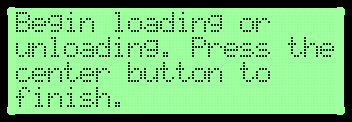
\includegraphics[]{load-04}
    \caption{Loading or Unloading}
  \label{fig:filpro}
\end{figure}

At this point you may manually load, unload, or change the filament.  The printer will automatically turn on the proper extruder's stepper motor, allowing the filament to be fed in or backed out.  Note that while pressing the center key will return you to the ``Filament Loading'' menu, pressing the left key will generate a screen asking if you wish to cancel.  To confirm the cancellation, select ``Yes'' and press the center key.

\NextFile{ui-utilities-menu-preheat-settings.html}

\subsection{Preheat Settings} \label{sec:preheatset}
\index{Preheat!Temperatures}
\index{Utilities!Preheat settings}
\index{Menus!Preheat settings}

This option allows you to set the preheat temperatures for each of the heating elements.  Temperatures are all in degrees Celsius.  This option displays the screen shown in Figure~\ref{fig:preset}.  As always, the number of extruders listed will depend on the number your printer has.

 \begin{figure}[!htbp]
  \centering
    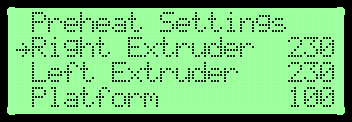
\includegraphics[]{preheat-settings-01}
    \caption{Preheat Setting}
  \label{fig:preset}
\end{figure}

To change the temperature for a heated element, select it and press the center key, then use the up key to increase the temperature and the down key to decrease it.  To save the changes to a temperature, press the center key.  The left key is used to exit the menu and return to ``Utilities''.  The maximum temperature that the firmware will allow you to set is 280\textdegree\,C for the extruders, and 130\textdegree\,C for the build platform.\index{Temperature!Maximums}

\NextFile{ui-utilities-menu-general-settings.html}

\subsection{General Settings} \label{sec:general}
\index{Utilities!General settings}
\index{Menus!General settings}

This menu allows you to change many simple settings.  The screen will show you up to four options at once.  To choose an option press the center key.  You may then use the up and down keys to toggle between two choices for that setting and press the center key to save the change.  The left key will exit the menu and return you to ``Utilities''.

\NextFile{ui-utilities-menu-general-settings-ditto-printing.html}

\subsubsection{Ditto Printing} \label{sec:ditto}
\index{Ditto printing}
\index{Printing!Ditto}
\index{Parameters!Ditto}

If you have more than one extruder, than this option allows you to reproduce the print for a second extruder, enabling you to print two of the same thing at once.  It does not matter for which extruder the print was sliced, it will be reproduced on both.  You do have to make sure that on no given layer will the two nozzles interfere with each other.  If you only have one extruder, this option will display the text ``N/A'' as it is unavailable.  By default, this feature is disabled. %clever ditto printing examples?

 \begin{figure}[!htbp]
  \centering
    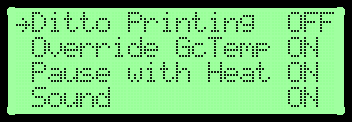
\includegraphics[]{general-01}
    \caption{General Settings --- First Screen}
  \label{fig:genfirst}
\end{figure}

\NextFile{ui-utilities-menu-general-settings-override-gctemp.html}

\subsubsection{Override GcTemp} \label{sec:override}
\index{Overriding temperatures}
\index{Temperature!Overriding}
\index{Printing!Overriding temperatures}
\index{Parameters!Override gcode temperature}

When enabled, this option allows you to override the non-zero temperatures in a print file.  These temperatures will be replaced by the preheat temperature for the given heater.  This is useful for experimentation or for switching plastics without reslicing.  By default, this feature is disabled.

\NextFile{ui-utilities-menu-general-settings-pause-with-heat.html}

\subsubsection{Pause with Heat} \label{sec:pauseheat}
\index{Pausing!Leaving heaters on}
\index{Parameters!Pause with heat}

If this option is enabled, it allows the heaters to remain on when a print is paused.  However, even if ``Pause with Heat'' is enabled the heaters will turn off after the print is paused for over 30 minutes due to safety reasons.  By default, this feature is disabled.

\NextFile{ui-utilities-menu-general-settings-sound.html}

\subsubsection{Sound} \label{sec:sound}
\index{Parameters!Sound}
\index{Buzzer}
\index{Sound}

If you are annoyed by the buzzer, use this option to turn it off.  The buzzer normally sounds when the printer turns on to tell you the firmware has started, the announcement of some warning messages is accompanied by the buzzer, and print files can include tunes played on the buzzer.  By default, this feature is enabled.

\NextFile{ui-utilities-menu-general-settings-acceleration.html}

\subsubsection{Acceleration} \label{sec:acceleration-enable}
\index{Parameters!Acceleration}
\index{Acceleration!Disabling}

This enables the printer's use of acceleration when effecting move commands.  When acceleration is disabled, the printer will attempt to instantaneously jump to the requested speeds, causing more jerks and vibrations.  If you wish to print with acceleration disabled, print at speeds closer to 30--40~mm/s, as printing at high speeds with acceleration disabled can both damage the printer as well as ruin your print.  By default, this feature is enabled.

 \begin{figure}[!htbp]
  \centering
    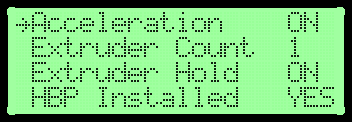
\includegraphics[]{general-02}
    \caption{General Settings --- Second Screen}
  \label{fig:gen2}
\end{figure}

\NextFile{ui-utilities-menu-general-settings-extruder-count.html}

\subsubsection{Extruder Count} \label{sec:extruder-count}
\index{Parameters!Extruder count}
\index{Tool count}
\index{Extruder count}

This tells the firmware the number of extruders with which your printer is equipped.  More than two extruders is not supported by standard Sailfish distributions.  The default extruder count depends on your type of printer.  The default is one for a Replicator 2, and two for all other printers.

After changing the extruder count, the printer should be power cycled for the change to take effect.

\NextFile{ui-utilities-menu-general-settings-extruder-hold.html}

\subsubsection{Extruder Hold} \label{sec:extruder-hold}
\index{Parameters!Extruder hold}

This is primarily meant for extruders that use 3 millimeter filament.  This ensures that, throughout the entire print, the extruder's stepper motor is kept engaged and does not allow the filament to creep out.  This is mostly a problem with extruders that accept 3 millimeter filament, as larger filament generates more back pressure.  Therefore, this option is intended to counteract the tendency of filament to back out of the extruder when the stepper motor is temporarily disabled, a command some \glspl{slicer} will add to the print command file (for instance, ReplicatorG).  For Cupcake printers the default is on; for all other printers, the default is off.

\NextFile{ui-utilities-menu-general-settings-hbp-installed.html}

\subsubsection{HBP Installed} \label{sec:hbp-present}
\index{Parameters!HBP installed}
\index{Heated build platform!Enabling}

This tells the firmware if your printer is equipped with a heated build platform.  The default is no for a Replicator 2, and yes for all other printers.

After changing the \gls{HBP} setting, the printer should be power cycled in order for the change to take effect.

\NextFile{ui-utilities-menu-general-settings-check-sd-reads.html}

\subsubsection{Check SD Reads} \label{sec:sd-crc}
\index{SD card!Error checking}
\index{SD card!CRC}
\index{Parameters!Check SD reads}

This allows you to check for errors when reading or writing to the SD card.  Typically, with this feature disabled, errors in reading or writing to the SD card may make the printer do something unexpected.  With this feature enabled, if an error is detected, the operation will be reattempted up to five times, at which point the print will be canceled.  Note that, enabling this feature this can affect performance when printing fine detail at high speeds.  By default, this feature is disabled.
 
 \begin{figure}[!htbp]
  \centering
    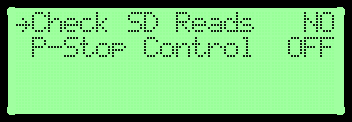
\includegraphics[]{general-03}
    \caption{General Settings --- Third Screen}
  \label{fig:gen3}
\end{figure}

\NextFile{ui-utilities-menu-general-settings-pstop-control.html}

\subsubsection{P-Stop Control} \label{sec:pstop-enable}
\index{Parameters!P-Stop}
\index{Pausing!P-Stop}
\index{Filament jam detector}
\index{P-Stop}

If you have equipped your printer with extra hardware (such as a filament jam detector) to trigger a build pause, then you will want to enable this feature.  When enabled, this allows extra hardware to tell the printer to pause a print, allowing you to fix any error condition and resume the print.  Do not enable this unless you have installed such hardware, as the printer will not function when it cannot detect any additional hardware.  Likewise, the extra hardware will be ignored if this is not enabled.  By default, this feature is disabled.

\NextFile{ui-utilities-menu-general-settings-serial-io.html}

\subsubsection{Serial I/O} \label{sec:alternate-uart}
\index{Parameters!Serial I/O}

Printers with ATmega~2560 microprocessors include an experimental option which allows all serial communications to be passed through the printer's alternate serial port, UART1, instead of the USB port.  When this option is set to the value ``UART1'' the USB port becomes non-functional: the printer will only communicate through the alternate serial port.

Presently, this option is being used by advanced users experimenting with Bluetooth, network, and other alternate forms of printer communications and control.  

\NextFile{ui-utilities-menu-level-build-plate.html}

\subsection{Level Build Plate} \label{sec:levelbp}
\index{Utilities!Level build plate}
\index{Leveling}

Choosing this option will home the axes, first X and Y, and then Z.  Once homed, the extruder will be moved to the center of the build plate, as defined in the ``Home Offsets'' section under the ``Utilities'' menu, Section~\ref{sec:homeoff}.  The X and Y stepper motors are then disabled, while the Z stepper motor is left enabled.

Now you can freely move the extruder to any position above the build plate in order to check if the build plate is level.  Sailfish does not require you to move the extruder to designated checkpoints, allowing you to go to the points you want to, in the order you want to, as many times as you want to.  

A screen will be generated explaining this procedure which may be dismissed by pressing the center key.  The fourth screen will tell you to press the center key to return to the ``Utilities'' menu and disengage the Z stepper motor when you are finished leveling the build plate.

\NextFile{ui-utilities-menu-home-axes.html}

\subsection{Home Axes} \label{sec:home-axes}
\index{Utilities!Home axes}
\index{Homing}

This is simply a convenience utility to home the axes for you.  This may be useful when diagnosing mechanical problems.

\NextFile{ui-utilities-menu-bot-statistics.html}

\subsection{Bot Statistics} \label{sec:bot-stats}
\index{Utilities!Bot statistics}
\index{Screens!Bot statistics}

This option displays usage information for your printer (Figure~\ref{fig:botstat}).

 \begin{figure}[!htbp]
  \centering
    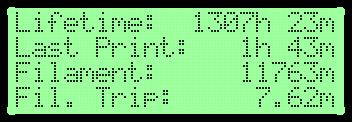
\includegraphics[]{botstats-01}
    \caption{Bot Statistics}
  \label{fig:botstat}
\end{figure}

\begin{enumerate}
\item The lifetime printing time in hours and minutes.\index{Printing!Lifetime usage}
\item The time spent on the last print in hours and minutes.\index{Printing!Last print time}
\item The lifetime filament length used in meters.\index{Filament!Usage}
\item The length of filament used since the filament trip odometer was last reset in meters or millimeters.  This can be reset in the ``Filament Odometer'' option under ``Utilities'', Section~\ref{sec:filodo}.\index{Printing!Filament last used}
\end{enumerate}

This menu may be exited by pressing either the center or left keys.

\NextFile{ui-utilities-menu-filament-odometer.html}

\subsection{Filament Odometer} \label{sec:filodo}
\index{Utilities!Filament odometer}
\index{Filament!Usage}
\index{Filament!Odometer}

This option shows a screen similar to the one depicted in Figure~\ref{fig:odo}.

 \begin{figure}[!htbp]
  \centering
    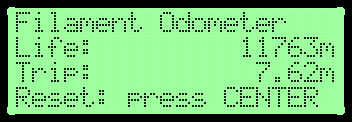
\includegraphics[]{odometer-01}
    \caption{Filament Odometer}
  \label{fig:odo}
\end{figure}

This displays the lifetime filament usage in meters or millimeters.  This also displays the amount of filament used since the filament trip odometer was last reset.  The odometer can be reset by pressing the center key.  To exit the menu, press the left key.

\NextFile{ui-utilities-menu-profiles.html}

\subsection{Profiles} \label{sec:profiles}
\index{Utilities!Profiles}
\index{Profiles}

This item lets you save up to four different sets of preheat and home offsets settings, and quickly recall them to enable ease of printing with different plastics, build surfaces, prints, slicers, etc.

The default names assigned to the profiles are ``ABS'', ``PLA'', ``Profile3'', and ``Profile4''.  You can change these names by selecting them, pressing the center key, and choosing the ``Change Name'' item of the profile
\ifpdf
menu.
\else
menu, Section~\ref{sec:profile-menu}.
\fi

\NextFile{ui-utilities-menu-profiles-profile-menu.html}

\subsubsection{Profile Menu} \label{sec:profile-menu}
\index{Menus!Profile}

Once you select one of the profiles, the profile menu will be generated.  It contains four items:

\begin{enumerate}
\item Restore:\label{sec:profiles-r} selecting this restores the saved home offsets and preheat temperatures, making them your current settings.  These settings will survive power cycles.  Selecting this will also return you to the ``Utilities'' menu, Section~\ref{sec:utilities}.
\item Display Config:\label{sec:profiles-dc} choosing this generates screens similar to the ones depicted in Figures~\ref{fig:cd1} and \ref{fig:cd2}.\index{Profiles!Displaying}

\begin{figure}[!htbp]
 \centering
    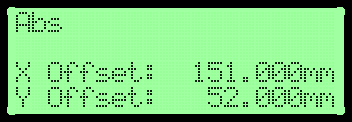
\includegraphics[]{profile-display-01}
    \caption{Configuration Display --- Screen 1}
  \label{fig:cd1}
\end{figure}

\begin{figure}[!htbp]
  \centering
    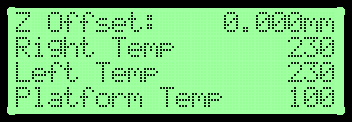
\includegraphics[]{profile-display-02}
    \caption{Configuration Display --- Screen 2}
  \label{fig:cd2}
\end{figure}

\item Change Name:\label{sec:profiles-cn} this allows you to change the name of a profile, using the interface similar to the one shown in Figure~\ref{fig:name}.\index{Profiles!Change name}

\begin{figure}[!htbp]
  \centering
    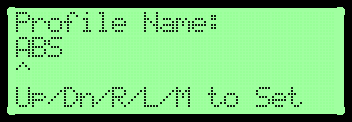
\includegraphics[]{profiles-name-01}
    \caption{Change Name}
  \label{fig:name}
\end{figure}

To change the letters, use the up and down keys.  To move between letters, use the left and right keys.  Press the center key to save all changes and return to the profile menu.  Note that if you are at the leftmost character (for example, the ``A'' in Figure~\ref{fig:name}) the left key will exit the menu without saving any changes.
\item Save to Profile:\label{sec:profiles-sp} selecting this saves your current home offsets and preheat settings to the selected profile and returns you to the ``Utilities'' menu.
\end{enumerate}

You can always save your current settings to a profile, replacing what is currently there.  This allows you to restore a profile, edit it in ``Preheat Settings'' (Section~\ref{sec:preheatset}) and ``Home Offsets'' (Section~\ref{sec:homeoff}) under the ``Utilities'' menu, and save it again.

\NextFile{ui-utilities-menu-home-offsets.html}

\subsection{Home Offsets} \label{sec:homeoff}
\index{Home offsets}
\index{Offsets!Home}
\index{Utilities!Home offsets}
\index{Menus!Home offsets}

This menu allows you to change the \glspl{home offset}, which define the center of the build plate (0,0,0) relative to the endstops.  For instance, if the X home offset is 152~mm, then the endstop is 152~mm to the right of the center.

This menu walks you through the three offsets, generating first the screen for the X offset (Figure~\ref{fig:xoff}).

 \begin{figure}[!htbp]
  \centering
    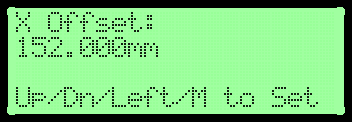
\includegraphics[]{offsets-01}
    \caption{X Offset}
  \label{fig:xoff}
\end{figure}

Pressing the up key increases the value, pressing the down key decreases the value.  The values are changed internally in units of steps and displayed to you in millimeters.  Press the left key to cancel any further changes, and the center key to confirm the change.  For example, if you only wish to adjust the X offset, press the center key to confirm the change for X and then press the left key to prevent any further changes.

\NextFile{ui-utilities-menu-toolhead-offsets.html}

\subsection{Toolhead Offsets} \label{sec:tooloff}
\index{Toolhead offsets}
\index{Offsets!Toolhead}
\index{Utilities!Toolhead offsets}
\index{Menus!Toolhead offsets}

This menu was added in Sailfish~7.7: you will not see it if you have an earlier version of Sailfish.  Additionally, this menu only appears for printers with an extruder count set to two as per Section~\ref{sec:extruder-count}.

With this menu, you can change the X and Y toolhead offsets which describe the spacing between the two extruder nozzles.  For a description of the toolhead offsets and how to calibrate them, see Section~\ref{sec:toolheadoffsets}.  Use of this menu is intended for when you wish to check the toolhead offsets or set their values in units of millimeters.  If instead you have printed the standard nozzle calibration print and are seeking to input the integer indices ranging from 1 to 13, then use the ``Calibrate Nozzles'' menu described in Section~\ref{sec:calibnozz}

The use and navigation of this menu is identical to that for the ``Home Offsets'' menu, with the exception that this menu only changes values for the X and Y axes.  See Section~\ref{sec:homeoff} for usage directions.

\NextFile{ui-utilities-menu-temp-sensor-types.html}

\subsection{Temperature Sensor Types} \label{sec:tempsensor}
\index{Temperature}

For users of Azteeg X3 electronics, this menu appears to allow you to set the type of temperature sensor used for the extruders and heated platform on your machine.

While MakerBot-style printers all use Type K thermocouples for the extruder temperature sensors and a specific 100K NTC thermistor for the heated bed, owners of Panucatt's Azteeg X3 electronics tend to use whatever temperature sensor is readily available.  As such, the Sailfish firmware builds for the Azteeg has a menu to select between seven different temperature sensors for the two extruders (Tool 0 and Tool 1) and the heated bed.  The choices are
\setlist[enumerate,1]{start=0}
\begin{enumerate}
\item K Thermocouple: Type K thermocouple
\item Generic 100K: Generic 100K NTC thermistor, beta 4338K
\item Semitec 204GT-2: 200K ATC Semitec 204GT-2 thermistor
\item Mendel: Mendel parts 100K thermistor
\item Generic 10K: Generic 10K NTC thermistor, beta xxxx
\item Semitec 104GT-2: 100K ATC Semitec 104GT-2 thermistor
\item Epcos 100K: Epcos 100K thermistor
\item Hw 135-104LAG-J01: Honeywell 135-104LAG-J01 thermistor
\end{enumerate}
\setlist[enumerate,1]{start=1}

As a default, the type is set to ``6.\ Epcos 100K'' as this thermistor is widely used.

After navigating into this menu, the up key can be used to increase the numeric designation and the down key can be used to decrease the numeric designation. Note that the list wraps. By pressing the left key, any further changes can be canceled and the menu exited. Pressing the center key confirms a change and advances to the next tool. In order, the menu asks you to set the two extruders (Tool 0 and Tool 1) and then the heated build platform.

\NextFile{ui-utilities-menu-jog-mode.html}

\subsection{Jog Mode} \label{sec:jog}
\index{Jogging}
\index{Utilities!Jog}
\index{Menus!Jogging}

This menu allows you to move the extruder and build plate.  When selected, the jog X screen should be generated.  You can navigate between the jog X, Y, and Z screens with the left and right keys.  The jog Y screen is shown in Figure~\ref{fig:jog} below.

\begin{figure}[!htbp]
  \centering
    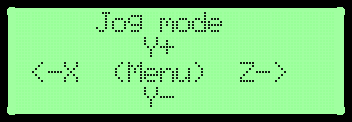
\includegraphics[]{jog-02}
    \caption{Jog Y}
  \label{fig:jog}
\end{figure}

As the screen shows, to increase the X, Y, or Z value press the up key, and press the down key to decrease the value.  The center key may be pressed to return you to the ``Utilities'' menu.  Note that +X is towards the right, +Y is towards the back, and +Z is towards the bottom.

\NextFile{ui-utilities-menu-enable-disable-steppers.html}

\subsection{Enable/Disable Steppers} \label{sec:steppers-enable}
\index{Stepper motors, enabling}
\index{Utilities!Enable steppers}
\index{Utilities!Disable steppers}

Selecting this will change the status of all stepper motors.  When they are enabled, they lock the axes in place.  Do not leave them enabled for extended periods of time as it heats up the motors needlessly.  By default, the stepper motors are disabled.

\NextFile{ui-utilities-menu-auto-level-adj.html}

\subsection{Auto-level Adjust} \label{sec:alevel-adj}
\index{Auto-leveling!Adjust}

Firmware assisted auto-leveling support was introduced in Sailfish~7.7 and 4.7 for all printers equipped with ATmega 2560 microprocessors. This parameter (see Figure ~\ref{fig:alevel-adj}) allows the user to specify ``deflection'' values indicating how much the build plate is deflected by the force of probing at each probe point (P1, P2, P3). 

\begin{figure}[!htbp]
  \centering
    \includegraphics[]{alevel-03}
    \caption{Auto-level Adjust}
  \label{fig:alevel-adj}
\end{figure}

For instance, a typically cantilevered build plate such as on a Replicator 1, 2, or 2X will be deflected downwards more the further the probe point is from the supporting Z rods. In this example, a probe point close to the Z rods might have a 0 mm deflection adjustment while points at the far edge may have deflections between 0.10 to 0.15 mm.� The auto-leveling code takes these deflection values into account as it calculates where the Z=0 plane truly lies.

This item allows you to see the deflection values for each of the three probe points, with the default being 0.00 mm. By using the up key to increase the value and the down key to decrease the value, you can set each deflection value to a positive or negative number. By pressing the center key you can set each value, and by pressing the left key you can cancel any change.

\NextFile{ui-utilities-menu-auto-level-variance.html}

\subsection{Auto-level Variance} \label{sec:alevel-variance}
\index{Auto-leveling!Max variance}

Firmware assisted auto-leveling support was introduced in Sailfish~7.7 and 4.7 for all printers equipped with ATmega 2560 microprocessors.  This parameter specifies the maximum tolerable difference in heights between the probing points.  If the difference in height between any two of the three probing points exceeds this parameter, then a print which attempts to enable auto-leveling will be canceled with the error message, ``Auto-level failed; too far out of level''.  Should that occur, it is time to manually relevel the build plate; see Section~\ref{sec:leveling}.

\begin{figure}[!htbp]
  \centering
    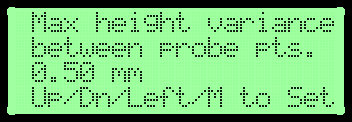
\includegraphics[]{alevel-01}
    \caption{Auto-level variance}
  \label{fig:alevel-variance}
\end{figure}

With this menu, depicted in Figure~\ref{fig:alevel-variance}, you can alter the value of this parameter.  The default value is 0.5~mm, and may be set to any value in the range 0.01 to 0.99~mm.  Pressing the up key increases the value, pressing the down key decreases the value.  Press the left key to cancel your changes; press the center key to confirm the change.

\NextFile{ui-utilities-menu-max-z-probe-hits.html}

\subsection{Max Z Probe Hits} \label{sec:alevel-maxhits}
\index{Auto-leveling!False probe hits}

When auto-leveling is active the Z height probe may be triggered by the ongoing build.  This might happen if over-extrusion is occurring, if the build has come loose, etc.  By default, the printer will initiate a pause and await user intervention when more than twenty triggers --- probe hits --- occur.  You may increase or decrease this value within the range of 1 to 200.  If you wish, you can disable this entirely by setting the ``max Z probe hits'' parameter to the value 0.  

\begin{figure}[!htbp]
  \centering
    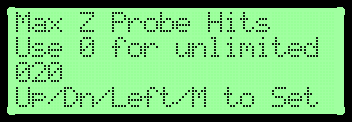
\includegraphics[]{alevel-02}
    \caption{Max Z probe hits}
  \label{fig:alevel-maxhits}
\end{figure}

To operate the menu, depicted in Figure~\ref{fig:alevel-maxhits}, press the up and down keys to increase or decrease the value.  To effect the change, press the center key.  To leave the menu without changing the setting, press the left key.

\NextFile{ui-utilities-menu-calibrate-nozzles.html}

\subsection{Calibrate Nozzles} \label{sec:calibnozz}
\index{Calibration!Dual extrusion|(}
This menu item is only available for printers with an extruder count set to two (see Section~\ref{sec:extruder-count}).

After you have run a nozzle calibration print, as described in Section~\ref{sec:dual-calib}, and having determined which of the thirteen X lines and which of the thirteen Y lines line up the best, this item allows you to enter their indices.  The firmware will take these indices and then compute and set the proper X and Y toolhead offsets.

It is important to note that \emph{these indices are not stored themselves}.  They are merely inputs used to compute the correct \emph{toolhead offsets} which \emph{are} stored.  Do not expect to return to this screen at a later date and see your values saved.  When you enter the screen you will always see the numbers 7 and 7, as they correspond to ideal nozzle spacings, as shown in Figure~\ref{fig:alignnozzles}.

\begin{figure}[!htbp]
  \centering
    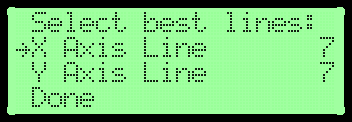
\includegraphics[]{align-01}
    \caption{Align Nozzles}
  \label{fig:alignnozzles}
\end{figure}

To change the values, press the center key to select the line and then use the up key to increase the value or the down key to decrease the value.  Note that the values range from one to thirteen and do not wrap.  Press the center key to save the change.  Either pressing the left key (when a line is not selected) or choosing the ``Done'' option returns you to the ``Utilities'' menu.
\index{Calibration!Dual extrusion|)}

\NextFile{ui-utilities-menu-cooling-fan-power.html}

\subsection{Cooling Fan Power} \label{sec:cfanpower}
\index{Utilities!Cooling fan power}
\index{Cooling fan}

This menu item allows you to set the strength of the cooling fan as a percentage of the total power. This setting is then used each time the print cooling fan is turned on.  Note that \glspl{X3G} lacks a power-level parameter for the FAN ON command, and therefore the fan's power level cannot be controlled by gcode.

To change the percentage, press the center key to select the item.  Use the up key to increase the value and the down key to decrease it.  The values range from 0 to 100\%, with 0\%\, being equivalent to off and 100\%\, being full power.  Note that the values do not wrap and increment by one. Also, the increment will increase the longer you hold the up or down key.  Press the center key to save the change and return to the ``Utilities'' menu. If you press the left key, you will cancel any change and be returned to the ``Utilities'' menu.

\NextFile{ui-utilities-menu-restore-settings.html}

\subsection{Restore Settings} \label{sec:restore-settings}
\index{Utilities!Restore settings}
\index{Factory defaults}
\index{Resetting the printer}

Selecting this option will generate a confirmation screen, as depicted in Figure~\ref{fig:restore} below.  Confirming the change will restore all factory settings save for the home offsets and toolhead offsets (Sections~\ref{sec:homeoff} and \ref{sec:tooloff}).  This will also save lifetime filament and print hours information.  If you wish to reset everything, see Section \ref{sec:eeprom}.

\begin{figure}[!htbp]
  \centering
    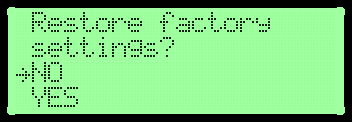
\includegraphics[]{restore-01}
    \caption{Restore Factory Settings}
  \label{fig:restore}
\end{figure}

\NextFile{ui-utilities-menu-eeprom.html}

\subsection{EEPROM} \label{sec:eeprom}
\index{Utilities!EEPROM}
\index{Menus!EEPROM}
\index{EEPROM}
\index{Resetting the printer}

\gls{EEPROM} stands for Electrically Erasable Programable Read-Only Memory.  Operational parameters for your printer, such as home offsets (Section~\ref{sec:homeoff}), preheat temperatures (Section~\ref{sec:preheatset}), etc.\ are saved in your EEPROM.\ \ Selecting this item generates a warning screen (Figure~\ref{fig:EEPROMwarning}), as, should you accidentally restore an EEPROM file from a different printer, you may make your printer inoperable.

\begin{figure}[!htbp]
  \centering
    
\includegraphics[]{eeprom-01}
    \caption{Use EEPROM With Care}
  \label{fig:EEPROMwarning}
\end{figure}

You may dismiss this screen by pressing the up key, which will generate the EEPROM menu, as shown in Figure~\ref{fig:eeprom}.  Pressing the left key will return you to the ``Utilities'' menu.

\begin{figure}[!htbp]
  \centering
    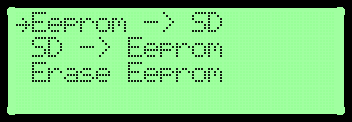
\includegraphics[]{eeprom-02}
    \caption{The EEPROM Menu}
  \label{fig:eeprom}
\end{figure}

This menu allows you to write your EEPROM to an SD card installed in your printer.  This creates a 4K file called \texttt{eeprom\textunderscore dump.bin} in the currently selected folder.\index{eeprom\textunderscore dump.bin@\texttt{eeprom\textunderscore dump.bin}}\index{EEPROM!Saving}  If this file already exists, an error message will be displayed and the transfer will not happen.  You may press the center key to dismiss the error message and return to the EEPROM menu.

The second item in the menu allows you to replace your EEPROM with the settings on your SD card (Figure \ref{fig:three}).  To successfully implement the settings on your SD card, you must press the center key a total of four times, at which point it will restore the file, and tell the printer to reset itself, returning you to the main menu, Section \ref{sec:Main}.\index{EEPROM!Restoring}

\begin{figure}[!htbp]
  \centering
    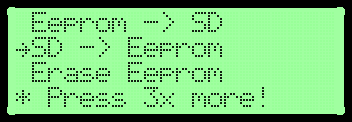
\includegraphics[]{eeprom-03}
    \caption{Due to the dangerous nature of restoring settings from an SD card, you are asked to confirm your selection of this item multiple times in order to prevent an accidental selection which may render your printer inoperable.}
  \label{fig:three}
\end{figure}

The final item in this menu (``Erase EEPROM'') will reinitialize the entire EEPROM memory.  Unlike the ``Restore Settings'' menu (Section~\ref{sec:restore-settings}), this item even resets the home and toolhead offsets, restoring \emph{all} factory defaults.

\NextFile{ui-utilities-menu-version-information.html}

\subsection{Version Information} \label{sec:versinf}
\index{Utilities!Version information}
\index{Screens!Version information}
\index{Version}
\index{Revision}
\index{Build date}

Selecting this item generates a screen similar to the one depicted in Figure~\ref{fig:vi}. 

\begin{figure}[!htbp]
  \centering
    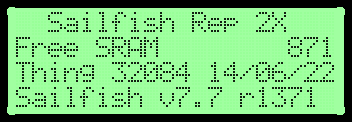
\includegraphics[]{version-01}
    \caption{Version Information}
  \label{fig:vi}
\end{figure}

This contains the following information:

\begin{enumerate}
\item The type of machine for which the firmware was compiled.  Hopefully this corresponds to the type of your printer.
\item The amount of free bytes of memory (RAM) that your printer has.  If this gets below 50, something is wrong with the firmware.\index{Memory usage}
\item The type of microprocessor, ATmega~1280 or 2560, in your printer.
\item The date the firmware was built in year/month/day format.
\item The version and revision numbers of the firmware.
\end{enumerate}
